\documentclass[lang=cn,11pt,a4paper,cite=authornum]{paper}

\title{编译原理与技术 实验二:语法分析程序的设计与实现 \\ 实验报告}
\author{毛子恒 \\ 2019211397}
\institute{北京邮电大学\ 计算机学院}

\date{\zhtoday}

% 本文档命令
\usepackage{array}
\newcommand{\ccr}[1]{\makecell{{\color{#1}\rule{1cm}{1cm}}}}
\nocite{*}

\begin{document}

\maketitle

\section{概览}

\subsection{任务描述}

编写语法分析程序,实现对算术表达式的语法分析。要求所分析算术表达式由如下的文法产生。

\label{grammar}
$$
\begin{aligned}
& E\rightarrow E+T | E-T | T \\
& T\rightarrow T*F | T/F | F \\
& F\rightarrow (E) | num
\end{aligned}
$$

要求在对输入的算术表达式进行分析的过程中,依次输出所采用的产生式。

编写LL(1)语法分析程序,要求如下:

\begin{enumerate}
    \item 为给定文法自动构造预测分析表。
    \item 构造LL(1)预测分析程序。
\end{enumerate}

\subsection{开发环境}

\begin{itemize}
    \item macOS Big Sur 11.6
    \item Apple clang version 12.0.5
    \item cmake version 3.19.6
    \item Clion 2021.2.1
    \item Visual Studio Code 1.61.2
\end{itemize}

\section{模块介绍}

\subsection{模块划分}

各模块及其关系如\figref{fig:structure}。

\begin{figure}[htbp]

    \centering
    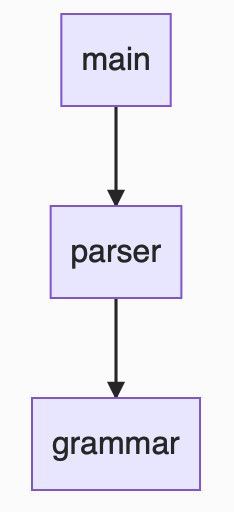
\includegraphics[width=0.15\linewidth]{./images/structure.png}
    \caption{模块关系图\label{fig:structure}}

\end{figure}

其中,\mintinline{text}{grammar}模块定义了文法类,其中实现了文法的输入,以及消除左递归、消除左公因子、计算FIRST和FOLLOW集的算法;\mintinline{text}{parser}模块定义了预测分析类,实现了从LL(1)文法构造预测分析表的构造函数,以及利用预测分析表分析字符串的方法。

主函数的流程如下:

\begin{itemize}
    \item 从文件中读入文法。
    \item 对文法进行转换并且判断是否是LL(1)文法。
    \item 利用文法构建预测分析表
    \item 从文件中读入需要分析的字符串。
    \item 对字符串进行预测分析,输出分析过程。
\end{itemize}

\subsection{文法类}

\mintinline{text}{grammar}模块中定义了文法类:

\begin{code}
\begin{minted}{C++}
using Symbol = std::string;
using SymbolSet = std::unordered_set<Symbol>;
using ProductionRight = std::deque<std::string>;
using Productions = std::unordered_map<Symbol, std::vector<ProductionRight>>;
class Grammar
{
public:
    Grammar();
    void LoadFromFile(std::ifstream &fs);
    bool ConvertToLL1();
    const SymbolSet &GetNonterminal() const;
    const SymbolSet &GetTerminal() const;
    const Productions &GetProduction() const;
    const Symbol &GetStart() const;
    const std::unordered_map<std::string, std::vector<SymbolSet>> &GetCandidateFirst() const;
    const std::unordered_map<std::string, SymbolSet> &GetFollow() const;
private:
    SymbolSet nonterminal;
    SymbolSet terminal;
    Productions production;
    Symbol start;
    std::unordered_map<std::string, std::vector<SymbolSet>> candidate_first;
    std::unordered_map<std::string, SymbolSet> first;
    std::unordered_map<std::string, SymbolSet> follow;
    void EliminateLeftRecursion();
    void EliminateLeftFactoring();
    void ConstructFirst(const Symbol &left);
    void ConstructFirstSet();
    void ConstructFollow(const Symbol &left, std::unordered_map<Symbol, std::unordered_map<Symbol, bool>> &include_follow);
    void ConstructFollowSet();
    bool IsLL1Grammar() const;
};
std::ostream &operator<<(std::ostream &os, const SymbolSet &rhs);
std::ostream &operator<<(std::ostream &os, const ProductionRight &rhs);
std::ostream &operator<<(std::ostream &os, const Productions &rhs);
\end{minted}
\end{code}

该类中包含有文法的非终结符号集合、终结符号集合、产生式集合、起始符号、候选式的FIRST集、非终结符的FIRST集合非终结符的FOLLOW集成员。

\subsubsection{文法的输入}

\mintinline{text}{LoadFromFile}方法实现了从一个文件输入流中读取文法,一个描述\ref{grammar}节中文法的文件示例如下:

\label{grammar_text}
\begin{code}
\begin{minted}{text}
$ Nonterminal symbols
E T F
$ Terminal symbols
+ - * / ( ) num
$ Start symbol
E
$ Productions
E -> E + T $ E - T $ T
T -> T * F $ T / F $ F
F -> ( E ) $ num
\end{minted}
\end{code}

文件依次输入非终结符号集合、终结符号集合、起始符号、文法产生式集合。每个部分的开始都以一行单独的说明字符串标识,各个部分均可包含多行,各个符号之间以空格分隔。产生式中以\mintinline{text}{$}符号代替\mintinline{text}{|}符号。

输入时,程序会对文法的合法性进行基本的判断,包括非终结符号集和终结符号集不重合、起始符号是非终结符号、产生式左部是非终结符号、右部是非终结符号或者终结符号。

\subsubsection{文法转换为LL(1)文法}

\mintinline{text}{ComvertToLL1}方法实现了将文法转换为LL(1)文法,该方法依次调用\mintinline{text}{EliminateLeftRecursion}、\mintinline{text}{EliminateLeftFactoring}、\mintinline{text}{ConstructFirstSet}、\mintinline{text}{ConstructFollowSet}、\mintinline{text}{IsLL1Grammar}方法,并在这期间输出调试信息。

\paragraph{消除左递归} \mintinline{text}{EliminateLeftRecursion}方法实现了消除左递归算法,即对于有如下产生式的非终结符$A$:

$$
A\rightarrow A\alpha_1|A\alpha_2|\ldots|A\alpha_n|\beta_1|\beta_2|\ldots|\beta_m
$$

其中,$\beta_i(i=1,2,\ldots,m)$不以$A$打头。用如下产生式替代:

$$
\begin{aligned}
& A\rightarrow \beta_1A'|\beta_2A'|\ldots|\beta_mA' \\
& A'\rightarrow \alpha_1A'|\alpha_2A'|\ldots|\alpha_nA'|\varepsilon
\end{aligned}
$$

该算法的伪代码见\algoref{algo:eli_left_recur}。

\begin{algorithm}[!htb]
    \caption{消除左递归\label{algo:eli_left_recur}}
    \KwIn{$\mathbf G = (\mathbf N, \mathbf T, \mathbf P, S)$}
    \KwOut{$\mathbf G_1 = (\mathbf N_1, \mathbf T, \mathbf P_1, S)$}
    \SetKwProg{Fn}{Function}{}{end}
    \SetKwData{P}{$\mathbf P$}
    \SetKwData{Po}{$\mathbf P_1$}
    \SetKwData{N}{$\mathbf N$}
    \SetKwData{No}{$\mathbf N_1$}
    \SetKwFunction{EliLeftRecur}{EliminateLeftRecursion}
    \Fn(){\EliLeftRecur{}}{
        $\Po\leftarrow \varnothing$\;
        $\No\leftarrow \N$\;
        \ForEach{$A\in \N$}{
            \If{$A\rightarrow A\alpha\not\in \P$}{
                \ForEach{$A\rightarrow\beta\in\P$}{
                    $\Po\leftarrow\Po\cup\{A\rightarrow\beta\}$\;
                }
            }
            \Else{
                $\No\leftarrow\No\cup\{A'\}$\;
                $\Po\leftarrow\Po\cup\{A\rightarrow\varepsilon\}$\;
                \ForEach{$A\rightarrow A\alpha\in\P$}{
                    $\Po\leftarrow\Po\cup\{A'\rightarrow\alpha A'\}$\;
                }
                \ForEach{$A\rightarrow \beta\in\P$}{
                    $\Po\leftarrow\Po\cup\{A\rightarrow\beta A'\}$\;
                }
            }
        }
    }
\end{algorithm}

\paragraph{消除左公因子} \mintinline{text}{EliminateLeftFactoring}方法实现了消除左公因子算法,即对于每个非终结符$A$,找出它的两个或更多候选式的最长公共前缀$\alpha$,如果$\alpha\not=\varepsilon$,有如下产生式:

$$
A\rightarrow \alpha\beta_1|\alpha\beta_2|\ldots|\alpha\beta_n|\gamma_1|\gamma_2|\ldots|\gamma_m
$$

其中,$\gamma_i(i=1,2,\ldots,m)$表示不以$\alpha$打头的表达式。用如下产生式替代:

$$
\begin{aligned}
& A\rightarrow \alpha A'|\gamma_1|\gamma_2|\ldots|\gamma_m \\
& A'\rightarrow \beta_1|\beta_2|\ldots|\beta_n
\end{aligned}
$$
该算法的伪代码见\algoref{algo:eli_left_fact}。

\begin{algorithm}[!htb]
    \caption{消除左公因子\label{algo:eli_left_fact}}
    \KwIn{$\mathbf G = (\mathbf N, \mathbf T, \mathbf P, S)$}
    \KwOut{$\mathbf G_1 = (\mathbf N_1, \mathbf T, \mathbf P_1, S)$}
    \SetKwProg{Fn}{Function}{}{end}
    \SetKwData{P}{$\mathbf P$}
    \SetKwData{Po}{$\mathbf P_1$}
    \SetKwData{Pz}{$\mathbf P_0$}
    \SetKwData{N}{$\mathbf N$}
    \SetKwData{No}{$\mathbf N_1$}
    \SetKwFunction{EliLeftFact}{EliminateLeftFactoring}
    \Fn(){\EliLeftFact{}}{
        $\Po\leftarrow \varnothing$\;
        $\No\leftarrow \N$\;
        \Do{$\Pz\not=\varnothing$}{
            $\Pz\leftarrow\varnothing$\;
            \ForEach{$A\in\N$}{
                \While{$\exists A\rightarrow\alpha\beta_1|\alpha\beta_2\in\P$}{
                    $\No\leftarrow\No\cup\{A'\}$\;
                    \ForEach{$A\rightarrow\alpha\beta_i\in\P$}{
                        $\P\leftarrow\P-\{A\rightarrow\alpha\beta_i\}$\;
                        $\Pz\leftarrow\Pz\cup\{A'\rightarrow\beta_i\}$\;
                    }
                    $\P\leftarrow\P\cup\{A\rightarrow\alpha A'\}$\;
                }
                \ForEach{$A\rightarrow\alpha\in\P$}{
                    $\P\leftarrow\P-\{A\rightarrow\alpha\}$\;
                    $\Po\leftarrow\Po\cup\{A\rightarrow\alpha\}$\;
                }
            }
        }
    }
\end{algorithm}

\paragraph{构建非终结符和候选式的FIRST集} \mintinline{text}{ConstructFirstSet}方法实现了构建非终结符和候选式的FIRST集,对于任意产生式$A\rightarrow\alpha$,若$\alpha\not=\varepsilon$,设该产生式为:

$$
A\rightarrow Y_1Y_2\ldots Y_k
$$

遍历产生式右部的每一个$Y_i$,如果:

\begin{itemize}
    \item $Y_i$是终结符,则$\alpha$的FIRST集中增加$Y_i$,终止遍历;
    \item $Y_i$是非终结符,如果没有求出它的FIRST集,则递归求解。之后,$\alpha$的FIRST集并上$Y_i$的FIRST集。此后检查$Y_i$的FIRST集中是否包含$\varepsilon$(即是否能推导出$\varepsilon$),若不包含,则终止遍历。
\end{itemize}

最后,$A$的FIRST集为各个候选式的FIRST集的并。

该算法的伪代码见\algoref{algo:cons_first}。

\begin{algorithm}[!htb]
    \caption{构建非终结符和候选式的FIRST集\label{algo:cons_first}}
    \KwIn{$\mathbf G = (\mathbf N, \mathbf T, \mathbf P, S)$}
    \KwOut{$\mathbf{FIRST}$}
    \SetKwProg{Fn}{Function}{}{end}
    \SetKwData{P}{$\mathbf P$}
    \SetKwData{N}{$\mathbf N$}
    \SetKwData{T}{$\mathbf T$}
    \SetKwData{FIRST}{$\mathbf{FIRST}$}
    \SetKwFunction{ConsFirst}{ConstructFirst}
    \SetKwFunction{ConsFirstSet}{ConstructFirstSet}
    \Fn(){\ConsFirst{A}}{
        \ForEach{$A\rightarrow\alpha\in\P$}{
            \If{$\alpha=\varepsilon$}{
                $\FIRST(A)\leftarrow\FIRST(A)\cup\{\varepsilon\}$\;
                $\FIRST(\alpha)\leftarrow\{\varepsilon\}$\;
            }
            \For(\tcp*[f]{$\alpha=Y_1Y_2\ldots Y_k$}){$i\leftarrow 1$ \KwTo $k$}{
                \If{$Y_i\in\T$}{
                    $\FIRST(\alpha)\leftarrow\FIRST(\alpha)\cup\{Y_i\}$\;
                    break\;
                }
                \lIf{$\FIRST(Y_i)=\varnothing$}{\ConsFirst{$Y_i$}}
                $\FIRST(\alpha)=\FIRST(\alpha)\cup\FIRST(Y_i)$\;
                \lIf{$\varepsilon\not\in\FIRST(Y_i)$}{break}
            }
            \lIf{$i=k$}{$\FIRST(A)\leftarrow\FIRST(A)\cup\{\varepsilon\}$}
            $\FIRST(A)\leftarrow\FIRST(A)\cup\FIRST(\alpha)$\;
        }
    }
    \Fn(){\ConsFirstSet{}}{
        \ForEach{$A\in\T$}{
            \lIf{$\FIRST(A)=\varnothing$}{\ConsFirst{$A$}}
        }
    }
\end{algorithm}

\paragraph{构建非终结符的FOLLOW集} \mintinline{text}{ConstructFollowSet}方法实现了构建非终结符的FOLLOW集,对于非终结符$B$,检查所有右部包含$B$的产生式$A\rightarrow\alpha BY_1Y_2\ldots Y_k$:

遍历每一个$Y_i$,如果:

\begin{itemize}
    \item $Y_i$是终结符,则$B$的FOLLOW集中增加$Y_i$,终止遍历;
    \item $Y_i$是非终结符,$B$的FOLLOW集并上$Y_i$的FIRST集中非空的部分。此后检查$Y_i$的FIRST集中是否包含$\varepsilon$(即是否能推导出$\varepsilon$),若不包含,则终止遍历。
\end{itemize}

如果遍历完$Y_k$并且$A\not=B$,则$A$的FOLLOW集包含在$B$的FOLLOW集中,为了处理两个非终结符的FOLLOW集互相包含导致无限递归的情况,采用\mintinline{text}{include_follow}变量记录非终结符的FOLLOW集的包含关系,以及\mintinline{text}{finished_construct_follow}变量记录FOLLOW集是否构建完成。如果一个非终结符$B$的FOLLOW集包含另一个终结符$A$的FOLLOW集,但是$A$的FOLLOW集不包含$B$的FOLLOW集并且$A$的FOLLOW集还没有处理,则可以递归处理$A$的FOLLOW集,完成后将$B$的FOLLOW集并上$A$的FOLLOW集。

在处理完所有非终结符的FOLLOW集后,处理两个集合相互包含(即两个集合相等)的情况,此时将两个集合都设为原本的集合的并即可。

该算法的伪代码见\algoref{algo:cons_follow}。

\begin{algorithm}[!htb]
    \caption{构建非终结符的FOLLOW集\label{algo:cons_follow}}
    \KwIn{$\mathbf G = (\mathbf N, \mathbf T, \mathbf P, S),\mathbf{FIRST}$}
    \KwOut{$\mathbf{FOLLOW}$}
    \SetKwProg{Fn}{Function}{}{end}
    \SetKwData{P}{$\mathbf P$}
    \SetKwData{T}{$\mathbf T$}
    \SetKwData{N}{$\mathbf N$}
    \SetKwData{FIRST}{$\mathbf{FIRST}$}
    \SetKwData{FOLLOW}{$\mathbf{FOLLOW}$}
    \SetKwData{ifol}{include\_follow}
    \SetKwData{fcfol}{finished\_construct\_follow}
    \SetKwFunction{ConsFol}{ConstructFollow}
    \SetKwFunction{ConsFolSet}{ConstructFollowSet}
    \Fn(){\ConsFol{B}}{
        \ForEach{$A\in\N$}{
            \ForEach{$A\rightarrow\alpha B\beta\in\P$}{
                \For(\tcp*[f]{$\beta=Y_1Y_2\ldots Y_k$}){$i\leftarrow 1$ \KwTo $k$}{
                    \If{$Y_i\in\T$}{
                        $\FOLLOW(B)\leftarrow\FOLLOW(B)\cup\{Y_i\}$\;
                        break\;
                    }
                    $\FOLLOW(B)\leftarrow\FOLLOW(B)\cup(\FIRST(Y_i)-\{\varepsilon\})$\;
                    \lIf{$\varepsilon\not\in\FIRST(Y_i)$}{break}
                }
                \If{$i=k \wedge A\not=B$}{
                    $\ifol[B,A]=true$\tcp*{$\FOLLOW(A)\subseteq \FOLLOW(B)$}
                    \If{$\ifol[A,B]=false\wedge\fcfol[A]=false$}{\ConsFol{A}\;}
                    $\FOLLOW(B)\leftarrow\FOLLOW(B)\cup\FOLLOW(A)$\;
                }
            }
        }
        $\fcfol[B]=true$\;
    }
    \Fn(){\ConsFolSet{}}{
        $\T\leftarrow\T\cup\{\$\}$\;
        $\FOLLOW(S)\leftarrow\{\$\}$\;
        \ForEach{$A\in\N$}{
            \lIf{$\FOLLOW(A)=\varnothing$}{\ConsFol{$A$}}
        }
        \ForEach{$A,B\in\N$}{
            \If{$\ifol[A,B]=true\wedge\ifol[B,A]=true$}{
                $\FOLLOW(A)\leftarrow\FOLLOW(A)\cup\FOLLOW(B)$\;
                $\FOLLOW(B)\leftarrow\FOLLOW(A)$\;
            }
        }
    }
\end{algorithm}

\paragraph{判断是否是LL(1)文法} \mintinline{text}{IsLL1Grammar}方法判断文法是否是LL(1)文法,即检查每个产生式$A\rightarrow\alpha|\beta$,需要满足:

\begin{itemize}
    \item $\mathbf{FIRST}(\alpha)\cap\mathbf{FIRST}(\beta)=\varnothing$
    \item 如果$A\rightarrow\varepsilon$,$\mathbf{FIRST}(\alpha)\cap\mathbf{FOLLOW}(A)=\varnothing$
\end{itemize}

\subsection{预测分析}

\mintinline{text}{parser}模块定义了预测分析类:

\begin{code}
\begin{minted}{C++}
using Production = std::pair<Symbol, ProductionRight>;
class Parser
{
public:
    Parser();
    explicit Parser(const Grammar &grammar);
    bool ParseString(const ProductionRight &str);
private:
    using Status = std::pair<std::vector<Symbol>, ProductionRight>;
    Symbol start;
    SymbolSet nonterminal;
    std::vector<Symbol> terminal;
    std::unordered_map<Symbol, std::unordered_map<Symbol, ProductionRight>> parsing_table;
    bool NextStep(Status &status, Production &production);
    friend std::ostream &operator<<(std::ostream &os, const Parser &rhs);
};
std::ostream &operator<<(std::ostream &os, const std::vector<Symbol> &rhs);
std::ostream &operator<<(std::ostream &os, const Production &rhs);
std::ostream &operator<<(std::ostream &os, const Parser &rhs);
\end{minted}
\end{code}

该类中的\mintinline{text}{parsing_table}为预测分析表。

\subsubsection{构建预测分析表}

\mintinline{text}{Parser(const Grammar &grammar)}构造函数通过LL(1)文法构造一个预测分析表,构造算法伪代码见\algoref{algo:cons_table}。

\begin{algorithm}[!htb]
    \caption{构建预测分析表\label{algo:cons_table}}
    \KwIn{$\mathbf G = (\mathbf N, \mathbf T, \mathbf P, S),\mathbf{FIRST},\mathbf{FOLLOW}$}
    \KwOut{预测分析表$\mathbf{M}$}
    \SetKwProg{Fn}{Function}{}{end}
    \SetKwData{P}{$\mathbf P$}
    \SetKwData{T}{$\mathbf T$}
    \SetKwData{Ma}{$\mathbf M$}
    \SetKwData{FIRST}{$\mathbf{FIRST}$}
    \SetKwData{FOLLOW}{$\mathbf{FOLLOW}$}
    \SetKwFunction{ConsTab}{ConstructParsingTable}
    \Fn(){\ConsTab{$\mathbf G$}}{
        \lForEach{$a\in\FIRST(\alpha)\cap\T$}{$\Ma[A,a]\leftarrow\{A\rightarrow\alpha\}$}
        \If{$\varepsilon\in\FIRST(\alpha)$}{
            \lForEach{$b\in\FOLLOW(A)$}{$\Ma[A,a]\leftarrow\{A\rightarrow\alpha\}$}
        }
        \lForEach{$\Ma[A,a]=\varnothing$}{$\Ma[A,a]=\{error\}$}
    }
\end{algorithm}

\subsubsection{预测分析算法}

\mintinline{text}{ParseString}方法实现对一个字符串的预测分析,该函数首先初始化一个状态,之后依照状态和当前字符串不返回断调用\mintinline{text}{NextStep}一步步进行预测分析,并且同时输出分析过程。该函数的返回值表示分析是否成功。

非递归预测算法的伪代码见\algoref{algo:parsing}。

\begin{algorithm}[!htb]
    \caption{非递归预测分析算法\label{algo:parsing}}
    \KwIn{输入符号串$\omega$,$\mathbf G = (\mathbf N, \mathbf T, \mathbf P, S)$及其预测分析表$\mathbf M$}
    \KwOut{若$\omega\in L(\mathbf{G})$,则输出$\omega$的最左推导$\mathsf{answer}$,否则报告错误}
    \SetKwProg{Fn}{Function}{}{end}
    \SetKwData{T}{$\mathbf T$}
    \SetKwData{Ma}{$\mathbf M$}
    \SetKwData{Stk}{stack}
    \SetKwData{Buf}{buffer}
    \SetKwData{Ip}{ip}
    \SetKwData{Ans}{answer}
    \SetKwFunction{Parse}{ParseString}
    \SetKwFunction{Push}{push}
    \SetKwFunction{Pop}{pop}
    \SetKwFunction{Top}{top}
    \SetKwFunction{Pb}{push\_back}
    \Fn(){\Parse{$\omega$}}{
        $\Stk.\Push(\$)$\;
        $\Stk.\Push(S)$\;
        $\Buf\leftarrow\omega\$$\;
        $\Ip\leftarrow 0$\;
        \Do{$X\not=\$$}{
            $X\leftarrow\Stk.\Top()$\;
            $a\leftarrow\Buf[\Ip]$\;
            \If{$X\in\T\cup\{\$\}$}{
                \If{$X=a$}{
                    $\Stk.\Pop()$\;
                    $\Ip\leftarrow\Ip+1$\;
                }
                \lElse{\KwRet{$error$}}
            }
            \Else{
                \If{$\Ma[X,a]=X\rightarrow Y_1Y_2\ldots Y_k$}{
                    $\Stk.\Pop()$\;
                    \lFor{$i\leftarrow k$ \KwTo $1$}{$\Stk.\Push(Y_i)$}
                    $\Ans.\Pb(X\rightarrow Y_1Y_2\ldots Y_k)$\;
                }
                \lElse{\KwRet{$error$}}
            }
        }
        \KwRet{$\Ans$}\;
    }
\end{algorithm}

\section{用户指南}

在项目目录中执行以下命令来编译:

\begin{code}
\begin{minted}{shell}
mkdir build
cd build
cmake ..
make
\end{minted}
\end{code}

编译完成后,运行:

\begin{code}
\begin{minted}{shell}
./Syntactic ../test/grammar.txt ../test/test1.txt
\end{minted}
\end{code}

运行截图如\figref{fig:running}所示。

\begin{figure}[htbp]

    \centering
    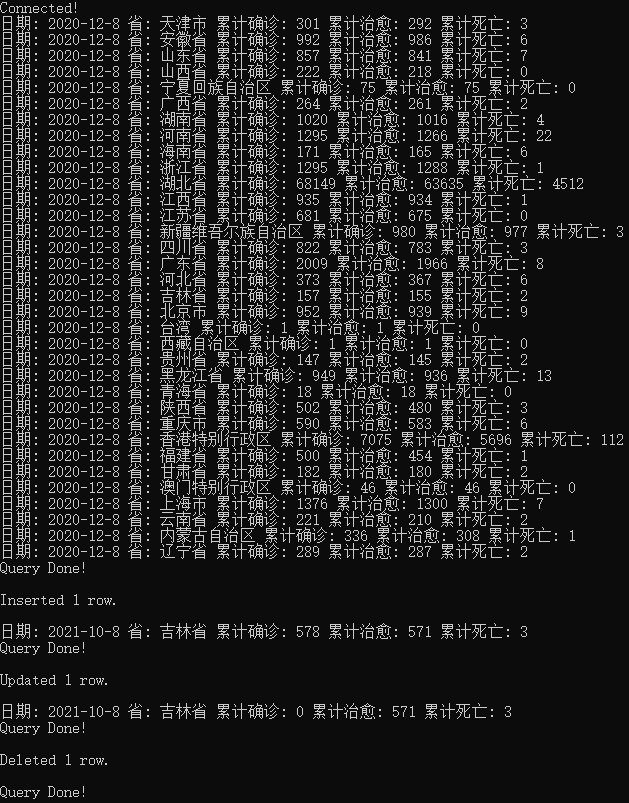
\includegraphics[width=0.7\linewidth]{./Images/running.png}
    \caption{运行截图\label{fig:running}}

\end{figure}

\section{测试结果}

\subsection{测试集1}

此测试集用于简单地测试程序是否正常运行。

\subsubsection{输入}

文法如\ref{grammar_text}节所示。

\begin{code}
\begin{minted}{text}
num + num
\end{minted}
\end{code}

\subsubsection{输出}

\begin{code}
\begin{minted}{text}
[Nonterminal Symbols] F T E 
[Terminal Symbols] * - ( num / ) + 
[Start Symbol] E
[Productions]
F -> ( E ) | num | 
T -> T * F | T / F | F | 
E -> E + T | E - T | T | 

[Nonterminal symbols] F T E' T' E 
[Terminal symbols] * - ( num / ) + 
[Start symbol] E
[Productions]
F -> ( E ) | num | 
T' -> [empty] | * F T' | / F T' | 
E' -> [empty] | + T E' | - T E' | 
E -> T E' | 
T -> F T' | 

[FIRST set of candidates]
Candidate      ( E ) 
FIRST          ( 
Candidate      num 
FIRST          num 
Candidate      F T' 
FIRST          ( num 
Candidate      [empty] 
FIRST          [empty] 
Candidate      + T E' 
FIRST          + 
Candidate      - T E' 
FIRST          - 
Candidate      [empty] 
FIRST          [empty] 
Candidate      * F T' 
FIRST          * 
Candidate      / F T' 
FIRST          / 
Candidate      T E' 
FIRST          ( num 

[FIRST and FOLLOW set of nonterminals]
Nonterminals   F
FIRST          num ( 
FOLLOW         - / $ + ) * 
Nonterminals   T
FIRST          num ( 
FOLLOW         ) + $ - 
Nonterminals   E'
FIRST          - + [empty] 
FOLLOW         $ ) 
Nonterminals   T'
FIRST          / * [empty] 
FOLLOW         - $ + ) 
Nonterminals   E
FIRST          num ( 
FOLLOW         ) $ 

[Parsing Table]
Nonterminal    E
    Terminal       (
    Production     E -> T E' 
    Terminal       num
    Production     E -> T E' 

Nonterminal    T'
    Terminal       *
    Production     T' -> * F T' 
    Terminal       -
    Production     T' -> [empty] 
    Terminal       $
    Production     T' -> [empty] 
    Terminal       /
    Production     T' -> / F T' 
    Terminal       )
    Production     T' -> [empty] 
    Terminal       +
    Production     T' -> [empty] 

Nonterminal    E'
    Terminal       -
    Production     E' -> - T E' 
    Terminal       $
    Production     E' -> [empty] 
    Terminal       )
    Production     E' -> [empty] 
    Terminal       +
    Production     E' -> + T E' 

Nonterminal    T
    Terminal       (
    Production     T -> F T' 
    Terminal       num
    Production     T -> F T' 

Nonterminal    F
    Terminal       (
    Production     F -> ( E ) 
    Terminal       num
    Production     F -> num 


Stack          $ E 
Input          num + num $ 
Output          

Stack          $ E' T 
Input          num + num $ 
Output         E -> T E' 

Stack          $ E' T' F 
Input          num + num $ 
Output         T -> F T' 

Stack          $ E' T' num 
Input          num + num $ 
Output         F -> num 

Stack          $ E' T' 
Input          + num $ 
Output         

Stack          $ E' 
Input          + num $ 
Output         T' -> [empty] 

Stack          $ E' T + 
Input          + num $ 
Output         E' -> + T E' 

Stack          $ E' T 
Input          num $ 
Output         

Stack          $ E' T' F 
Input          num $ 
Output         T -> F T' 

Stack          $ E' T' num 
Input          num $ 
Output         F -> num 

Stack          $ E' T' 
Input          $ 
Output         

Stack          $ E' 
Input          $ 
Output         T' -> [empty] 

Stack          $ 
Input          $ 
Output         E' -> [empty] 

Parsing successful!
\end{minted}
\end{code}

\subsubsection{分析}

程序首先输出原文法,之后输出消除左递归和左公因子的文法、候选式的FIRST集、非终结符的FIRST集和FOLLOW集、预测分析表。最后程序给出了分析字符串的过程。

\subsection{测试集2}

此测试集测试一个复杂的算术表达式。

\subsubsection{输入}

文法如\ref{grammar_text}节所示。

\begin{code}
\begin{minted}{text}
( num * ( ( ( ( num + num ) * num ) + num / num ) - num * ( num + num ) ) / num )
\end{minted}
\end{code}

\subsubsection{输出(部分)}

\begin{code}
\begin{minted}{text}
...

Stack          $ E 
Input          ( num * ( ( ( ( num + num ) * num ) + num / num ) - num * ( num + num ) ) / num ) $ 
Output          

Stack          $ E' T 
Input          ( num * ( ( ( ( num + num ) * num ) + num / num ) - num * ( num + num ) ) / num ) $ 
Output         E -> T E' 

Stack          $ E' T' F 
Input          ( num * ( ( ( ( num + num ) * num ) + num / num ) - num * ( num + num ) ) / num ) $ 
Output         T -> F T' 

Stack          $ E' T' ) E ( 
Input          ( num * ( ( ( ( num + num ) * num ) + num / num ) - num * ( num + num ) ) / num ) $ 
Output         F -> ( E ) 

Stack          $ E' T' ) E 
Input          num * ( ( ( ( num + num ) * num ) + num / num ) - num * ( num + num ) ) / num ) $ 
Output         

Stack          $ E' T' ) E' T 
Input          num * ( ( ( ( num + num ) * num ) + num / num ) - num * ( num + num ) ) / num ) $ 
Output         E -> T E' 

Stack          $ E' T' ) E' T' F 
Input          num * ( ( ( ( num + num ) * num ) + num / num ) - num * ( num + num ) ) / num ) $ 
Output         T -> F T' 

Stack          $ E' T' ) E' T' num 
Input          num * ( ( ( ( num + num ) * num ) + num / num ) - num * ( num + num ) ) / num ) $ 
Output         F -> num 

Stack          $ E' T' ) E' T' 
Input          * ( ( ( ( num + num ) * num ) + num / num ) - num * ( num + num ) ) / num ) $ 
Output         

Stack          $ E' T' ) E' T' F * 
Input          * ( ( ( ( num + num ) * num ) + num / num ) - num * ( num + num ) ) / num ) $ 
Output         T' -> * F T' 

Stack          $ E' T' ) E' T' F 
Input          ( ( ( ( num + num ) * num ) + num / num ) - num * ( num + num ) ) / num ) $ 
Output         

Stack          $ E' T' ) E' T' ) E ( 
Input          ( ( ( ( num + num ) * num ) + num / num ) - num * ( num + num ) ) / num ) $ 
Output         F -> ( E ) 

Stack          $ E' T' ) E' T' ) E 
Input          ( ( ( num + num ) * num ) + num / num ) - num * ( num + num ) ) / num ) $ 
Output         

Stack          $ E' T' ) E' T' ) E' T 
Input          ( ( ( num + num ) * num ) + num / num ) - num * ( num + num ) ) / num ) $ 
Output         E -> T E' 

Stack          $ E' T' ) E' T' ) E' T' F 
Input          ( ( ( num + num ) * num ) + num / num ) - num * ( num + num ) ) / num ) $ 
Output         T -> F T' 

Stack          $ E' T' ) E' T' ) E' T' ) E ( 
Input          ( ( ( num + num ) * num ) + num / num ) - num * ( num + num ) ) / num ) $ 
Output         F -> ( E ) 

Stack          $ E' T' ) E' T' ) E' T' ) E 
Input          ( ( num + num ) * num ) + num / num ) - num * ( num + num ) ) / num ) $ 
Output         

Stack          $ E' T' ) E' T' ) E' T' ) E' T 
Input          ( ( num + num ) * num ) + num / num ) - num * ( num + num ) ) / num ) $ 
Output         E -> T E' 

Stack          $ E' T' ) E' T' ) E' T' ) E' T' F 
Input          ( ( num + num ) * num ) + num / num ) - num * ( num + num ) ) / num ) $ 
Output         T -> F T' 

Stack          $ E' T' ) E' T' ) E' T' ) E' T' ) E ( 
Input          ( ( num + num ) * num ) + num / num ) - num * ( num + num ) ) / num ) $ 
Output         F -> ( E ) 

Stack          $ E' T' ) E' T' ) E' T' ) E' T' ) E 
Input          ( num + num ) * num ) + num / num ) - num * ( num + num ) ) / num ) $ 
Output         

Stack          $ E' T' ) E' T' ) E' T' ) E' T' ) E' T 
Input          ( num + num ) * num ) + num / num ) - num * ( num + num ) ) / num ) $ 
Output         E -> T E' 

Stack          $ E' T' ) E' T' ) E' T' ) E' T' ) E' T' F 
Input          ( num + num ) * num ) + num / num ) - num * ( num + num ) ) / num ) $ 
Output         T -> F T' 

Stack          $ E' T' ) E' T' ) E' T' ) E' T' ) E' T' ) E ( 
Input          ( num + num ) * num ) + num / num ) - num * ( num + num ) ) / num ) $ 
Output         F -> ( E ) 

Stack          $ E' T' ) E' T' ) E' T' ) E' T' ) E' T' ) E 
Input          num + num ) * num ) + num / num ) - num * ( num + num ) ) / num ) $ 
Output         

Stack          $ E' T' ) E' T' ) E' T' ) E' T' ) E' T' ) E' T 
Input          num + num ) * num ) + num / num ) - num * ( num + num ) ) / num ) $ 
Output         E -> T E' 

Stack          $ E' T' ) E' T' ) E' T' ) E' T' ) E' T' ) E' T' F 
Input          num + num ) * num ) + num / num ) - num * ( num + num ) ) / num ) $ 
Output         T -> F T' 

Stack          $ E' T' ) E' T' ) E' T' ) E' T' ) E' T' ) E' T' num 
Input          num + num ) * num ) + num / num ) - num * ( num + num ) ) / num ) $ 
Output         F -> num 

Stack          $ E' T' ) E' T' ) E' T' ) E' T' ) E' T' ) E' T' 
Input          + num ) * num ) + num / num ) - num * ( num + num ) ) / num ) $ 
Output         

Stack          $ E' T' ) E' T' ) E' T' ) E' T' ) E' T' ) E' 
Input          + num ) * num ) + num / num ) - num * ( num + num ) ) / num ) $ 
Output         T' -> [empty] 

Stack          $ E' T' ) E' T' ) E' T' ) E' T' ) E' T' ) E' T + 
Input          + num ) * num ) + num / num ) - num * ( num + num ) ) / num ) $ 
Output         E' -> + T E' 

Stack          $ E' T' ) E' T' ) E' T' ) E' T' ) E' T' ) E' T 
Input          num ) * num ) + num / num ) - num * ( num + num ) ) / num ) $ 
Output         

Stack          $ E' T' ) E' T' ) E' T' ) E' T' ) E' T' ) E' T' F 
Input          num ) * num ) + num / num ) - num * ( num + num ) ) / num ) $ 
Output         T -> F T' 

Stack          $ E' T' ) E' T' ) E' T' ) E' T' ) E' T' ) E' T' num 
Input          num ) * num ) + num / num ) - num * ( num + num ) ) / num ) $ 
Output         F -> num 

Stack          $ E' T' ) E' T' ) E' T' ) E' T' ) E' T' ) E' T' 
Input          ) * num ) + num / num ) - num * ( num + num ) ) / num ) $ 
Output         

Stack          $ E' T' ) E' T' ) E' T' ) E' T' ) E' T' ) E' 
Input          ) * num ) + num / num ) - num * ( num + num ) ) / num ) $ 
Output         T' -> [empty] 

Stack          $ E' T' ) E' T' ) E' T' ) E' T' ) E' T' ) 
Input          ) * num ) + num / num ) - num * ( num + num ) ) / num ) $ 
Output         E' -> [empty] 

Stack          $ E' T' ) E' T' ) E' T' ) E' T' ) E' T' 
Input          * num ) + num / num ) - num * ( num + num ) ) / num ) $ 
Output         

Stack          $ E' T' ) E' T' ) E' T' ) E' T' ) E' T' F * 
Input          * num ) + num / num ) - num * ( num + num ) ) / num ) $ 
Output         T' -> * F T' 

Stack          $ E' T' ) E' T' ) E' T' ) E' T' ) E' T' F 
Input          num ) + num / num ) - num * ( num + num ) ) / num ) $ 
Output         

Stack          $ E' T' ) E' T' ) E' T' ) E' T' ) E' T' num 
Input          num ) + num / num ) - num * ( num + num ) ) / num ) $ 
Output         F -> num 

Stack          $ E' T' ) E' T' ) E' T' ) E' T' ) E' T' 
Input          ) + num / num ) - num * ( num + num ) ) / num ) $ 
Output         

Stack          $ E' T' ) E' T' ) E' T' ) E' T' ) E' 
Input          ) + num / num ) - num * ( num + num ) ) / num ) $ 
Output         T' -> [empty] 

Stack          $ E' T' ) E' T' ) E' T' ) E' T' ) 
Input          ) + num / num ) - num * ( num + num ) ) / num ) $ 
Output         E' -> [empty] 

Stack          $ E' T' ) E' T' ) E' T' ) E' T' 
Input          + num / num ) - num * ( num + num ) ) / num ) $ 
Output         

Stack          $ E' T' ) E' T' ) E' T' ) E' 
Input          + num / num ) - num * ( num + num ) ) / num ) $ 
Output         T' -> [empty] 

Stack          $ E' T' ) E' T' ) E' T' ) E' T + 
Input          + num / num ) - num * ( num + num ) ) / num ) $ 
Output         E' -> + T E' 

Stack          $ E' T' ) E' T' ) E' T' ) E' T 
Input          num / num ) - num * ( num + num ) ) / num ) $ 
Output         

Stack          $ E' T' ) E' T' ) E' T' ) E' T' F 
Input          num / num ) - num * ( num + num ) ) / num ) $ 
Output         T -> F T' 

Stack          $ E' T' ) E' T' ) E' T' ) E' T' num 
Input          num / num ) - num * ( num + num ) ) / num ) $ 
Output         F -> num 

Stack          $ E' T' ) E' T' ) E' T' ) E' T' 
Input          / num ) - num * ( num + num ) ) / num ) $ 
Output         

Stack          $ E' T' ) E' T' ) E' T' ) E' T' F / 
Input          / num ) - num * ( num + num ) ) / num ) $ 
Output         T' -> / F T' 

Stack          $ E' T' ) E' T' ) E' T' ) E' T' F 
Input          num ) - num * ( num + num ) ) / num ) $ 
Output         

Stack          $ E' T' ) E' T' ) E' T' ) E' T' num 
Input          num ) - num * ( num + num ) ) / num ) $ 
Output         F -> num 

Stack          $ E' T' ) E' T' ) E' T' ) E' T' 
Input          ) - num * ( num + num ) ) / num ) $ 
Output         

Stack          $ E' T' ) E' T' ) E' T' ) E' 
Input          ) - num * ( num + num ) ) / num ) $ 
Output         T' -> [empty] 

Stack          $ E' T' ) E' T' ) E' T' ) 
Input          ) - num * ( num + num ) ) / num ) $ 
Output         E' -> [empty] 

Stack          $ E' T' ) E' T' ) E' T' 
Input          - num * ( num + num ) ) / num ) $ 
Output         

Stack          $ E' T' ) E' T' ) E' 
Input          - num * ( num + num ) ) / num ) $ 
Output         T' -> [empty] 

Stack          $ E' T' ) E' T' ) E' T - 
Input          - num * ( num + num ) ) / num ) $ 
Output         E' -> - T E' 

Stack          $ E' T' ) E' T' ) E' T 
Input          num * ( num + num ) ) / num ) $ 
Output         

Stack          $ E' T' ) E' T' ) E' T' F 
Input          num * ( num + num ) ) / num ) $ 
Output         T -> F T' 

Stack          $ E' T' ) E' T' ) E' T' num 
Input          num * ( num + num ) ) / num ) $ 
Output         F -> num 

Stack          $ E' T' ) E' T' ) E' T' 
Input          * ( num + num ) ) / num ) $ 
Output         

Stack          $ E' T' ) E' T' ) E' T' F * 
Input          * ( num + num ) ) / num ) $ 
Output         T' -> * F T' 

Stack          $ E' T' ) E' T' ) E' T' F 
Input          ( num + num ) ) / num ) $ 
Output         

Stack          $ E' T' ) E' T' ) E' T' ) E ( 
Input          ( num + num ) ) / num ) $ 
Output         F -> ( E ) 

Stack          $ E' T' ) E' T' ) E' T' ) E 
Input          num + num ) ) / num ) $ 
Output         

Stack          $ E' T' ) E' T' ) E' T' ) E' T 
Input          num + num ) ) / num ) $ 
Output         E -> T E' 

Stack          $ E' T' ) E' T' ) E' T' ) E' T' F 
Input          num + num ) ) / num ) $ 
Output         T -> F T' 

Stack          $ E' T' ) E' T' ) E' T' ) E' T' num 
Input          num + num ) ) / num ) $ 
Output         F -> num 

Stack          $ E' T' ) E' T' ) E' T' ) E' T' 
Input          + num ) ) / num ) $ 
Output         

Stack          $ E' T' ) E' T' ) E' T' ) E' 
Input          + num ) ) / num ) $ 
Output         T' -> [empty] 

Stack          $ E' T' ) E' T' ) E' T' ) E' T + 
Input          + num ) ) / num ) $ 
Output         E' -> + T E' 

Stack          $ E' T' ) E' T' ) E' T' ) E' T 
Input          num ) ) / num ) $ 
Output         

Stack          $ E' T' ) E' T' ) E' T' ) E' T' F 
Input          num ) ) / num ) $ 
Output         T -> F T' 

Stack          $ E' T' ) E' T' ) E' T' ) E' T' num 
Input          num ) ) / num ) $ 
Output         F -> num 

Stack          $ E' T' ) E' T' ) E' T' ) E' T' 
Input          ) ) / num ) $ 
Output         

Stack          $ E' T' ) E' T' ) E' T' ) E' 
Input          ) ) / num ) $ 
Output         T' -> [empty] 

Stack          $ E' T' ) E' T' ) E' T' ) 
Input          ) ) / num ) $ 
Output         E' -> [empty] 

Stack          $ E' T' ) E' T' ) E' T' 
Input          ) / num ) $ 
Output         

Stack          $ E' T' ) E' T' ) E' 
Input          ) / num ) $ 
Output         T' -> [empty] 

Stack          $ E' T' ) E' T' ) 
Input          ) / num ) $ 
Output         E' -> [empty] 

Stack          $ E' T' ) E' T' 
Input          / num ) $ 
Output         

Stack          $ E' T' ) E' T' F / 
Input          / num ) $ 
Output         T' -> / F T' 

Stack          $ E' T' ) E' T' F 
Input          num ) $ 
Output         

Stack          $ E' T' ) E' T' num 
Input          num ) $ 
Output         F -> num 

Stack          $ E' T' ) E' T' 
Input          ) $ 
Output         

Stack          $ E' T' ) E' 
Input          ) $ 
Output         T' -> [empty] 

Stack          $ E' T' ) 
Input          ) $ 
Output         E' -> [empty] 

Stack          $ E' T' 
Input          $ 
Output         

Stack          $ E' 
Input          $ 
Output         T' -> [empty] 

Stack          $ 
Input          $ 
Output         E' -> [empty] 

Parsing successful!
\end{minted}
\end{code}

\subsubsection{分析}

正确分析了此字符串。

\subsection{测试集3}

此测试集用于测试一个错误的算术表达式。

\subsubsection{输入}

文法如\ref{grammar_text}节所示。

\begin{code}
\begin{minted}{text}
( num + num ) * / num
\end{minted}
\end{code}

\subsubsection{输出(部分)}

\begin{code}
\begin{minted}{text}
...

Stack          $ E 
Input          ( num + num ) * / num $ 
Output          

Stack          $ E' T 
Input          ( num + num ) * / num $ 
Output         E -> T E' 

Stack          $ E' T' F 
Input          ( num + num ) * / num $ 
Output         T -> F T' 

Stack          $ E' T' ) E ( 
Input          ( num + num ) * / num $ 
Output         F -> ( E ) 

Stack          $ E' T' ) E 
Input          num + num ) * / num $ 
Output         

Stack          $ E' T' ) E' T 
Input          num + num ) * / num $ 
Output         E -> T E' 

Stack          $ E' T' ) E' T' F 
Input          num + num ) * / num $ 
Output         T -> F T' 

Stack          $ E' T' ) E' T' num 
Input          num + num ) * / num $ 
Output         F -> num 

Stack          $ E' T' ) E' T' 
Input          + num ) * / num $ 
Output         

Stack          $ E' T' ) E' 
Input          + num ) * / num $ 
Output         T' -> [empty] 

Stack          $ E' T' ) E' T + 
Input          + num ) * / num $ 
Output         E' -> + T E' 

Stack          $ E' T' ) E' T 
Input          num ) * / num $ 
Output         

Stack          $ E' T' ) E' T' F 
Input          num ) * / num $ 
Output         T -> F T' 

Stack          $ E' T' ) E' T' num 
Input          num ) * / num $ 
Output         F -> num 

Stack          $ E' T' ) E' T' 
Input          ) * / num $ 
Output         

Stack          $ E' T' ) E' 
Input          ) * / num $ 
Output         T' -> [empty] 

Stack          $ E' T' ) 
Input          ) * / num $ 
Output         E' -> [empty] 

Stack          $ E' T' 
Input          * / num $ 
Output         

Stack          $ E' T' F * 
Input          * / num $ 
Output         T' -> * F T' 

Stack          $ E' T' F 
Input          / num $ 
Output         

Parsing failed!
\end{minted}
\end{code}

\subsubsection{分析}

在分析到错误的\mintinline{text}{/}符号时,由于预测分析表中没有对应的项,分析程序报错并退出。

\subsection{测试集4}

此测试集用于测试一个错误的算术表达式。

\subsubsection{输入}

文法如\ref{grammar_text}节所示。

\begin{code}
\begin{minted}{text}
( ( num + num ) / num
\end{minted}
\end{code}

\subsubsection{输出(部分)}

\begin{code}
\begin{minted}{text}
...

Stack          $ E 
Input          ( ( num + num ) / num $ 
Output          

Stack          $ E' T 
Input          ( ( num + num ) / num $ 
Output         E -> T E' 

Stack          $ E' T' F 
Input          ( ( num + num ) / num $ 
Output         T -> F T' 

Stack          $ E' T' ) E ( 
Input          ( ( num + num ) / num $ 
Output         F -> ( E ) 

Stack          $ E' T' ) E 
Input          ( num + num ) / num $ 
Output         

Stack          $ E' T' ) E' T 
Input          ( num + num ) / num $ 
Output         E -> T E' 

Stack          $ E' T' ) E' T' F 
Input          ( num + num ) / num $ 
Output         T -> F T' 

Stack          $ E' T' ) E' T' ) E ( 
Input          ( num + num ) / num $ 
Output         F -> ( E ) 

Stack          $ E' T' ) E' T' ) E 
Input          num + num ) / num $ 
Output         

Stack          $ E' T' ) E' T' ) E' T 
Input          num + num ) / num $ 
Output         E -> T E' 

Stack          $ E' T' ) E' T' ) E' T' F 
Input          num + num ) / num $ 
Output         T -> F T' 

Stack          $ E' T' ) E' T' ) E' T' num 
Input          num + num ) / num $ 
Output         F -> num 

Stack          $ E' T' ) E' T' ) E' T' 
Input          + num ) / num $ 
Output         

Stack          $ E' T' ) E' T' ) E' 
Input          + num ) / num $ 
Output         T' -> [empty] 

Stack          $ E' T' ) E' T' ) E' T + 
Input          + num ) / num $ 
Output         E' -> + T E' 

Stack          $ E' T' ) E' T' ) E' T 
Input          num ) / num $ 
Output         

Stack          $ E' T' ) E' T' ) E' T' F 
Input          num ) / num $ 
Output         T -> F T' 

Stack          $ E' T' ) E' T' ) E' T' num 
Input          num ) / num $ 
Output         F -> num 

Stack          $ E' T' ) E' T' ) E' T' 
Input          ) / num $ 
Output         

Stack          $ E' T' ) E' T' ) E' 
Input          ) / num $ 
Output         T' -> [empty] 

Stack          $ E' T' ) E' T' ) 
Input          ) / num $ 
Output         E' -> [empty] 

Stack          $ E' T' ) E' T' 
Input          / num $ 
Output         

Stack          $ E' T' ) E' T' F / 
Input          / num $ 
Output         T' -> / F T' 

Stack          $ E' T' ) E' T' F 
Input          num $ 
Output         

Stack          $ E' T' ) E' T' num 
Input          num $ 
Output         F -> num 

Stack          $ E' T' ) E' T' 
Input          $ 
Output         

Stack          $ E' T' ) E' 
Input          $ 
Output         T' -> [empty] 

Stack          $ E' T' ) 
Input          $ 
Output         E' -> [empty] 

Parsing failed!
\end{minted}
\end{code}

\subsubsection{分析}

当分析到字符串尾时,由于栈顶的终结符和输入的符号不匹配,故分析程序报错并退出。

\subsection{测试集5}

此测试集依照习题4.5修改而来。

\subsubsection{输入}

\begin{code}
\begin{minted}{text}
$ Nonterminal symbols
E A B L
$ Terminal symbols
num id ( )
$ Start symbol
E
$ Productions
E -> A $ B
A -> num $ id
B -> ( L )
L -> L E $ E
\end{minted}
\end{code}

\begin{code}
\begin{minted}{text}
( id ( id ( num ) ) ( id ) )
\end{minted}
\end{code}

\subsubsection{输出}

\begin{code}
\begin{minted}{text}
[Nonterminal Symbols] L B A E 
[Terminal Symbols] ) ( id num 
[Start Symbol] E
[Productions]
L -> L E | E | 
B -> ( L ) | 
A -> num | id | 
E -> A | B | 

[Nonterminal symbols] L L' B A E 
[Terminal symbols] ) ( id num 
[Start symbol] E
[Productions]
L' -> [empty] | E L' | 
B -> ( L ) | 
L -> E L' | 
A -> num | id | 
E -> A | B | 

[FIRST set of candidates]
Candidate      E L' 
FIRST          num id ( 
Candidate      [empty] 
FIRST          [empty] 
Candidate      E L' 
FIRST          num id ( 
Candidate      ( L ) 
FIRST          ( 
Candidate      num 
FIRST          num 
Candidate      id 
FIRST          id 
Candidate      A 
FIRST          num id 
Candidate      B 
FIRST          ( 

[FIRST and FOLLOW set of nonterminals]
Nonterminals   L
FIRST          ( id num 
FOLLOW         ) 
Nonterminals   L'
FIRST          ( id num [empty] 
FOLLOW         ) 
Nonterminals   B
FIRST          ( 
FOLLOW         ( id num $ ) 
Nonterminals   A
FIRST          id num 
FOLLOW         ( id num $ ) 
Nonterminals   E
FIRST          ( id num 
FOLLOW         ) $ num id ( 

[Parsing Table]
Nonterminal    E
    Terminal       (
    Production     E -> B 
    Terminal       id
    Production     E -> A 
    Terminal       num
    Production     E -> A 

Nonterminal    A
    Terminal       id
    Production     A -> id 
    Terminal       num
    Production     A -> num 

Nonterminal    B
    Terminal       (
    Production     B -> ( L ) 

Nonterminal    L'
    Terminal       )
    Production     L' -> [empty] 
    Terminal       (
    Production     L' -> E L' 
    Terminal       id
    Production     L' -> E L' 
    Terminal       num
    Production     L' -> E L' 

Nonterminal    L
    Terminal       (
    Production     L -> E L' 
    Terminal       id
    Production     L -> E L' 
    Terminal       num
    Production     L -> E L' 


Stack          $ E 
Input          ( id ( id ( num ) ) ( id ) ) $ 
Output          

Stack          $ B 
Input          ( id ( id ( num ) ) ( id ) ) $ 
Output         E -> B 

Stack          $ ) L ( 
Input          ( id ( id ( num ) ) ( id ) ) $ 
Output         B -> ( L ) 

Stack          $ ) L 
Input          id ( id ( num ) ) ( id ) ) $ 
Output         

Stack          $ ) L' E 
Input          id ( id ( num ) ) ( id ) ) $ 
Output         L -> E L' 

Stack          $ ) L' A 
Input          id ( id ( num ) ) ( id ) ) $ 
Output         E -> A 

Stack          $ ) L' id 
Input          id ( id ( num ) ) ( id ) ) $ 
Output         A -> id 

Stack          $ ) L' 
Input          ( id ( num ) ) ( id ) ) $ 
Output         

Stack          $ ) L' E 
Input          ( id ( num ) ) ( id ) ) $ 
Output         L' -> E L' 

Stack          $ ) L' B 
Input          ( id ( num ) ) ( id ) ) $ 
Output         E -> B 

Stack          $ ) L' ) L ( 
Input          ( id ( num ) ) ( id ) ) $ 
Output         B -> ( L ) 

Stack          $ ) L' ) L 
Input          id ( num ) ) ( id ) ) $ 
Output         

Stack          $ ) L' ) L' E 
Input          id ( num ) ) ( id ) ) $ 
Output         L -> E L' 

Stack          $ ) L' ) L' A 
Input          id ( num ) ) ( id ) ) $ 
Output         E -> A 

Stack          $ ) L' ) L' id 
Input          id ( num ) ) ( id ) ) $ 
Output         A -> id 

Stack          $ ) L' ) L' 
Input          ( num ) ) ( id ) ) $ 
Output         

Stack          $ ) L' ) L' E 
Input          ( num ) ) ( id ) ) $ 
Output         L' -> E L' 

Stack          $ ) L' ) L' B 
Input          ( num ) ) ( id ) ) $ 
Output         E -> B 

Stack          $ ) L' ) L' ) L ( 
Input          ( num ) ) ( id ) ) $ 
Output         B -> ( L ) 

Stack          $ ) L' ) L' ) L 
Input          num ) ) ( id ) ) $ 
Output         

Stack          $ ) L' ) L' ) L' E 
Input          num ) ) ( id ) ) $ 
Output         L -> E L' 

Stack          $ ) L' ) L' ) L' A 
Input          num ) ) ( id ) ) $ 
Output         E -> A 

Stack          $ ) L' ) L' ) L' num 
Input          num ) ) ( id ) ) $ 
Output         A -> num 

Stack          $ ) L' ) L' ) L' 
Input          ) ) ( id ) ) $ 
Output         

Stack          $ ) L' ) L' ) 
Input          ) ) ( id ) ) $ 
Output         L' -> [empty] 

Stack          $ ) L' ) L' 
Input          ) ( id ) ) $ 
Output         

Stack          $ ) L' ) 
Input          ) ( id ) ) $ 
Output         L' -> [empty] 

Stack          $ ) L' 
Input          ( id ) ) $ 
Output         

Stack          $ ) L' E 
Input          ( id ) ) $ 
Output         L' -> E L' 

Stack          $ ) L' B 
Input          ( id ) ) $ 
Output         E -> B 

Stack          $ ) L' ) L ( 
Input          ( id ) ) $ 
Output         B -> ( L ) 

Stack          $ ) L' ) L 
Input          id ) ) $ 
Output         

Stack          $ ) L' ) L' E 
Input          id ) ) $ 
Output         L -> E L' 

Stack          $ ) L' ) L' A 
Input          id ) ) $ 
Output         E -> A 

Stack          $ ) L' ) L' id 
Input          id ) ) $ 
Output         A -> id 

Stack          $ ) L' ) L' 
Input          ) ) $ 
Output         

Stack          $ ) L' ) 
Input          ) ) $ 
Output         L' -> [empty] 

Stack          $ ) L' 
Input          ) $ 
Output         

Stack          $ ) 
Input          ) $ 
Output         L' -> [empty] 

Stack          $ 
Input          $ 
Output         

Parsing successful!
\end{minted}
\end{code}

\subsection{测试集6}

此测试集依照习题4.6修改而来。

\subsubsection{输入}

\begin{code}
\begin{minted}{text}
$ Nonterminal symbols
E A B L
$ Terminal symbols
num id ( ) ,
$ Start symbol
E
$ Productions
E -> A $ B
A -> num $ id
B -> ( L )
L -> L , E $ E
\end{minted}
\end{code}

\begin{code}
\begin{minted}{text}
( id , ( id ,  ( num ) ) , ( id ) )
\end{minted}
\end{code}

\subsubsection{输出}

\begin{code}
\begin{minted}{text}
[Nonterminal Symbols] L B A E 
[Terminal Symbols] , ) ( id num 
[Start Symbol] E
[Productions]
L -> L , E | E | 
B -> ( L ) | 
A -> num | id | 
E -> A | B | 

[Nonterminal symbols] L L' B A E 
[Terminal symbols] , ) ( id num 
[Start symbol] E
[Productions]
L' -> [empty] | , E L' | 
B -> ( L ) | 
L -> E L' | 
A -> num | id | 
E -> A | B | 

[FIRST set of candidates]
Candidate      E L' 
FIRST          num id ( 
Candidate      [empty] 
FIRST          [empty] 
Candidate      , E L' 
FIRST          , 
Candidate      ( L ) 
FIRST          ( 
Candidate      num 
FIRST          num 
Candidate      id 
FIRST          id 
Candidate      A 
FIRST          num id 
Candidate      B 
FIRST          ( 

[FIRST and FOLLOW set of nonterminals]
Nonterminals   L
FIRST          ( id num 
FOLLOW         ) 
Nonterminals   L'
FIRST          , [empty] 
FOLLOW         ) 
Nonterminals   B
FIRST          ( 
FOLLOW         $ , ) 
Nonterminals   A
FIRST          id num 
FOLLOW         $ , ) 
Nonterminals   E
FIRST          ( id num 
FOLLOW         ) , $ 

[Parsing Table]
Nonterminal    E
    Terminal       (
    Production     E -> B 
    Terminal       id
    Production     E -> A 
    Terminal       num
    Production     E -> A 

Nonterminal    A
    Terminal       id
    Production     A -> id 
    Terminal       num
    Production     A -> num 

Nonterminal    B
    Terminal       (
    Production     B -> ( L ) 

Nonterminal    L'
    Terminal       ,
    Production     L' -> , E L' 
    Terminal       )
    Production     L' -> [empty] 

Nonterminal    L
    Terminal       (
    Production     L -> E L' 
    Terminal       id
    Production     L -> E L' 
    Terminal       num
    Production     L -> E L' 


Stack          $ E 
Input          ( id , ( id , ( num ) ) , ( id ) ) $ 
Output          

Stack          $ B 
Input          ( id , ( id , ( num ) ) , ( id ) ) $ 
Output         E -> B 

Stack          $ ) L ( 
Input          ( id , ( id , ( num ) ) , ( id ) ) $ 
Output         B -> ( L ) 

Stack          $ ) L 
Input          id , ( id , ( num ) ) , ( id ) ) $ 
Output         

Stack          $ ) L' E 
Input          id , ( id , ( num ) ) , ( id ) ) $ 
Output         L -> E L' 

Stack          $ ) L' A 
Input          id , ( id , ( num ) ) , ( id ) ) $ 
Output         E -> A 

Stack          $ ) L' id 
Input          id , ( id , ( num ) ) , ( id ) ) $ 
Output         A -> id 

Stack          $ ) L' 
Input          , ( id , ( num ) ) , ( id ) ) $ 
Output         

Stack          $ ) L' E , 
Input          , ( id , ( num ) ) , ( id ) ) $ 
Output         L' -> , E L' 

Stack          $ ) L' E 
Input          ( id , ( num ) ) , ( id ) ) $ 
Output         

Stack          $ ) L' B 
Input          ( id , ( num ) ) , ( id ) ) $ 
Output         E -> B 

Stack          $ ) L' ) L ( 
Input          ( id , ( num ) ) , ( id ) ) $ 
Output         B -> ( L ) 

Stack          $ ) L' ) L 
Input          id , ( num ) ) , ( id ) ) $ 
Output         

Stack          $ ) L' ) L' E 
Input          id , ( num ) ) , ( id ) ) $ 
Output         L -> E L' 

Stack          $ ) L' ) L' A 
Input          id , ( num ) ) , ( id ) ) $ 
Output         E -> A 

Stack          $ ) L' ) L' id 
Input          id , ( num ) ) , ( id ) ) $ 
Output         A -> id 

Stack          $ ) L' ) L' 
Input          , ( num ) ) , ( id ) ) $ 
Output         

Stack          $ ) L' ) L' E , 
Input          , ( num ) ) , ( id ) ) $ 
Output         L' -> , E L' 

Stack          $ ) L' ) L' E 
Input          ( num ) ) , ( id ) ) $ 
Output         

Stack          $ ) L' ) L' B 
Input          ( num ) ) , ( id ) ) $ 
Output         E -> B 

Stack          $ ) L' ) L' ) L ( 
Input          ( num ) ) , ( id ) ) $ 
Output         B -> ( L ) 

Stack          $ ) L' ) L' ) L 
Input          num ) ) , ( id ) ) $ 
Output         

Stack          $ ) L' ) L' ) L' E 
Input          num ) ) , ( id ) ) $ 
Output         L -> E L' 

Stack          $ ) L' ) L' ) L' A 
Input          num ) ) , ( id ) ) $ 
Output         E -> A 

Stack          $ ) L' ) L' ) L' num 
Input          num ) ) , ( id ) ) $ 
Output         A -> num 

Stack          $ ) L' ) L' ) L' 
Input          ) ) , ( id ) ) $ 
Output         

Stack          $ ) L' ) L' ) 
Input          ) ) , ( id ) ) $ 
Output         L' -> [empty] 

Stack          $ ) L' ) L' 
Input          ) , ( id ) ) $ 
Output         

Stack          $ ) L' ) 
Input          ) , ( id ) ) $ 
Output         L' -> [empty] 

Stack          $ ) L' 
Input          , ( id ) ) $ 
Output         

Stack          $ ) L' E , 
Input          , ( id ) ) $ 
Output         L' -> , E L' 

Stack          $ ) L' E 
Input          ( id ) ) $ 
Output         

Stack          $ ) L' B 
Input          ( id ) ) $ 
Output         E -> B 

Stack          $ ) L' ) L ( 
Input          ( id ) ) $ 
Output         B -> ( L ) 

Stack          $ ) L' ) L 
Input          id ) ) $ 
Output         

Stack          $ ) L' ) L' E 
Input          id ) ) $ 
Output         L -> E L' 

Stack          $ ) L' ) L' A 
Input          id ) ) $ 
Output         E -> A 

Stack          $ ) L' ) L' id 
Input          id ) ) $ 
Output         A -> id 

Stack          $ ) L' ) L' 
Input          ) ) $ 
Output         

Stack          $ ) L' ) 
Input          ) ) $ 
Output         L' -> [empty] 

Stack          $ ) L' 
Input          ) $ 
Output         

Stack          $ ) 
Input          ) $ 
Output         L' -> [empty] 

Stack          $ 
Input          $ 
Output         

Parsing successful!
\end{minted}
\end{code}

\section{实验总结}

本次实验中我编写了一个LL(1)语法分析程序,使我对语法分析的流程更加清楚,对相关知识点的掌握更加牢固。

此程序的架构比较简单,主要难点在算法设计方面。对于语法分析中涉及的算法,尤其是消除左公因子和求FOLLOW集的算法,书上的介绍比较简单,手算和代码实现的差距比较大。

在成功实现这些算法并且通过测试之后,我尝试再次尝试编写了伪代码,这将会为我未来解题带来很大帮助。
在实现期间,我使用了C++的语法特性,使得维护文法产生式和预测分析表等变得更加容易,大大减少编程复杂度。

此外,我的语法分析程序仍然存在许多待改进的地方,比如分析错误时可以输出更多的报错信息、在进行文法转换和求解集合时的鲁棒性仍然有待提高,由于时间所限,这些情况我无法一一考虑周全。

本次实验除了让我对课内知识有了更多的认识,也使我的C++编程能力得到提高,我从中收获颇丰。

\end{document}